\chapter{Switches}

\section{Switch Terminology}

There are a few basic terms that get used with switches all the time.

Normally Open means that when the switch is in its normal position, the contacts are not touching, or open. Normally closed means that when the switch is in its normal position, the contacts are touching, or closed.

Single Throw means there's only two contacts. The switch is open or closed. Dual Throw means there's at least three contacts, and switching the switch moves the center contact from being closed with one outer contact to being closed with the other outer contact.

Single Throw means there's only one ser of contacts being closed or open by the switch's mechanism. Dual Throw means there's two sets of contacts being controlled by the same mechanism. With a dual throw switch, you can switch two separate circuits with the same mechanism.

\subsection{There are lots of types of switches.}

A few types are shown here:

\begin{figure}[!htb]
 \centering
 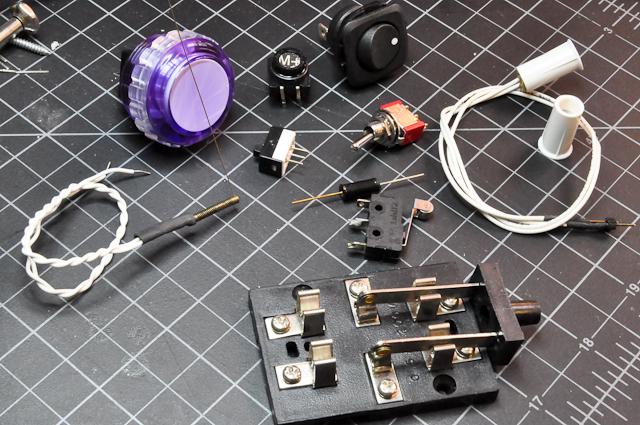
\includegraphics[scale=0.3]{img/switches/switches.jpg}
 \caption{various types of switches}
 \label{various types of switches}
\end{figure}

Pushbuttons or momentary switches stay closed only as long as you hold them closed. Roller switches are pushbuttons with a lever and a roller attached. They're useful when you need something to push against the switch gently to close it.

\begin{figure}[!htb]
 \centering
 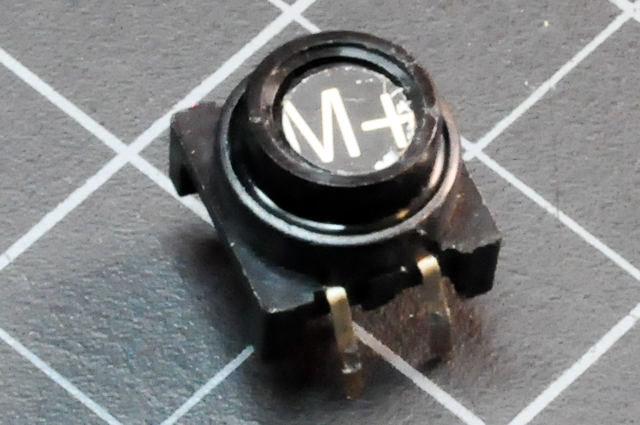
\includegraphics[scale=0.3]{img/switches/pushbutton.jpg}
 \caption{pushbutton}
 \label{pushbutton}
\end{figure}

\begin{figure}[!htb]
 \centering
 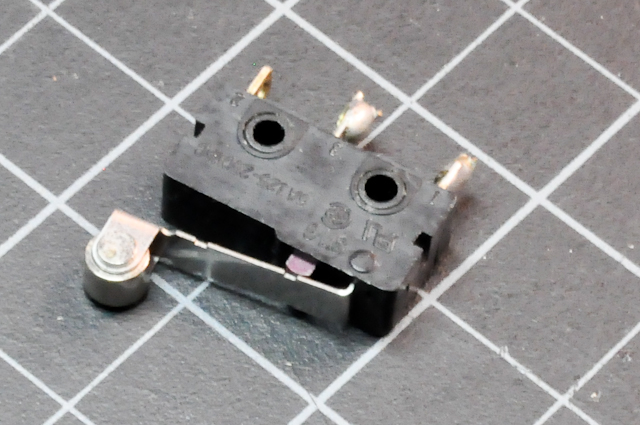
\includegraphics[scale=0.3]{img/switches/roller_switch.jpg}
 \caption{roller switch}
 \label{roller switch}
\end{figure}

Toggle switches stay closed in one physical position and open in the other. Slide switches are similar to toggle switches.

\begin{figure}[!htb]
 \centering
 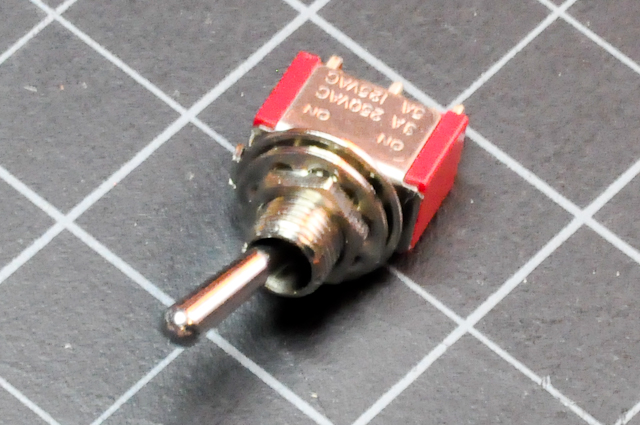
\includegraphics[scale=0.3]{img/switches/toggle_switch.jpg}
 \caption{toggle switch}
 \label{toggle switch}
\end{figure}

\begin{figure}[!htb]
 \centering
 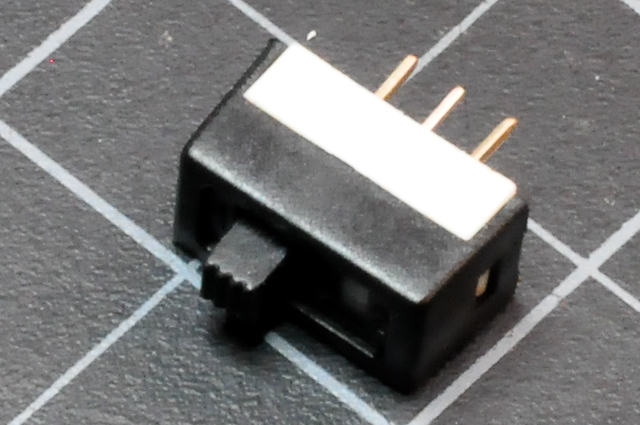
\includegraphics[scale=0.3]{img/switches/slide_switch.jpg}
 \caption{slide switch}
 \label{slide switch}
\end{figure}

Magnetic switches have two metal leaves in the end that are pulled together when a magnet is brought close to them. They're useful when you can't have wires on both sides of the switch mechanism.

\begin{figure}[!htb]
 \centering
 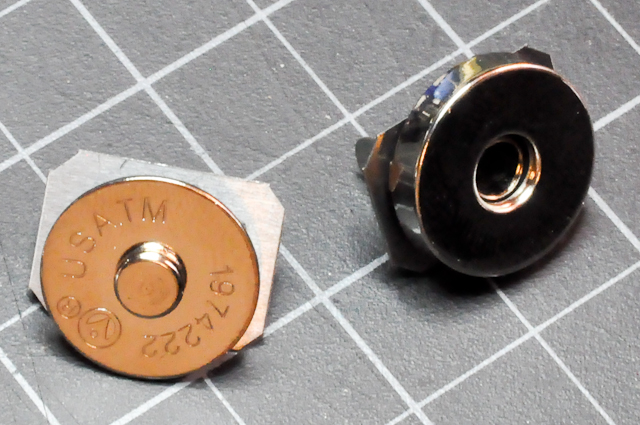
\includegraphics[scale=0.3]{img/switches/magnetic_snap.jpg}
 \caption{magnetic snap}
 \label{magnetic snap}
\end{figure}

Magnetic snaps are useful when you're making a soft circuit and need a fastener on the garment to close a switch.

Magnetic Snap

Whisker switches are made from a piece of spring steel or piano wire, and a center post. An insulator such as a piece of electrical tape or shrinkwrap holds the two separate. When the wire is touched, the spring bends and touches the metal post, and closes the switch. Solarbotics sells some nice whisker switches.

Whisker Switch

Tilt switches contain a metal ball and contacts at one end. When you tilt the switch, the ball touches both contacts, and closes the switch. There are also mercury switches that do the same, but with a ball of mercury inside. Avoid these, since mercury is very poisonous.

Whisker Switch

\section{Get Creative With Switches}

A switch is nothing more than a mechanism to bring two pieces of conductive material together and separate them. You can make a switch from any two conductors and a little creativity. Consider, for example:

conductive fabric

wire mesh

copper tape

All you need to do is arrange the two conductors in such a way that they can touch or not touch. Sometimes a spacer layered between the two conductors helps. For example, in this image you see three pieces of conductive fabric. Two of the pieces have non-conductive layers on top of them. When the non-conductive part is sandwiched between the conductive layers, you've got a switch that's pressed by touching. The conductive parts touch when they're pressed through the holes in the non-conductive part. These two switches would have different sensitivities because the hole-to-material ratio of the non-conductive layer is different.

soft switches

Make your own switch. Find a way to turn a closing door into a switch, for example, or to close a switch when a person sits down. Or figure out how to turn a hat into a switch, or a cane, or a zipper. Or perhaps the pieces of a puzzle can be switches.

Come up with an everyday activity to which you can add three or four custom switches that, when combined, turn on a light. For example, maybe the light comes on when you close the door, sit down, and open a book. Or when you walk upstairs, put your keys on a side table, and remove your hat. Combine your creativity with switches with what you learned in the electronics lab to make this happen.

For more ideas on materials, check out How to Get What You Want. They have an excellent list of conductive materials and instructions.

\section{Arrangements of switches}

In planning your switch project, consider what happens when you arrange switches in different ways. For example, try this circuit:

\subsection{Three switches in parallel. Any one of the three will turn on the LED}


Switches in parallel -- schematic

Switches in parallel -- breadboard

\subsection{Three switches in series. All three must be on to turn on the LED}


Switches in series -- schematic

Switches in series -- breadboard

Through a combination of series and parallel switches, you can come up with a variety of combinations that make the light turn on. Depending on where you add the LEDs, you can even have the same switches turn on different LEDs in different combinations. Try a few combinations and see what happens.

\begin{figure}[!htb]
 \centering
 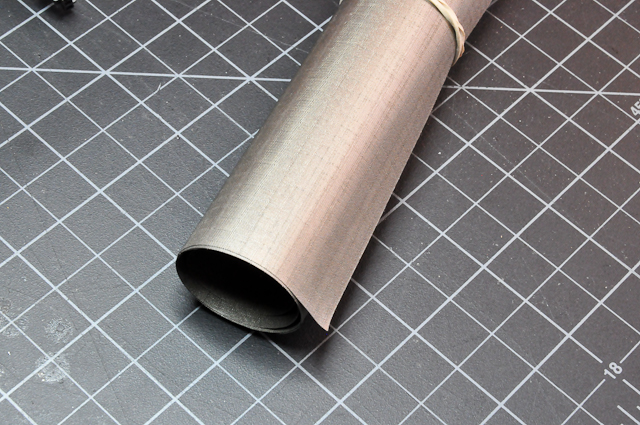
\includegraphics[scale=0.3]{img/switches/conductive_fabric.jpg}
 \caption{conductive fabric}
 \label{conductive fabric}
\end{figure}


\begin{figure}[!htb]
 \centering
 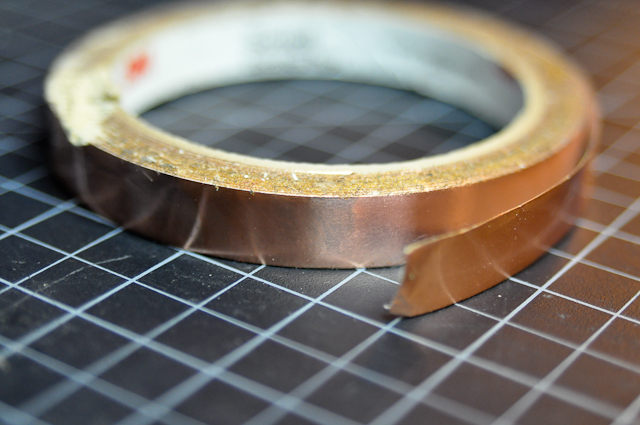
\includegraphics[scale=0.3]{img/switches/copper_tape.jpg}
 \caption{copper tape}
 \label{copper tape}
\end{figure}





\begin{figure}[!htb]
 \centering
 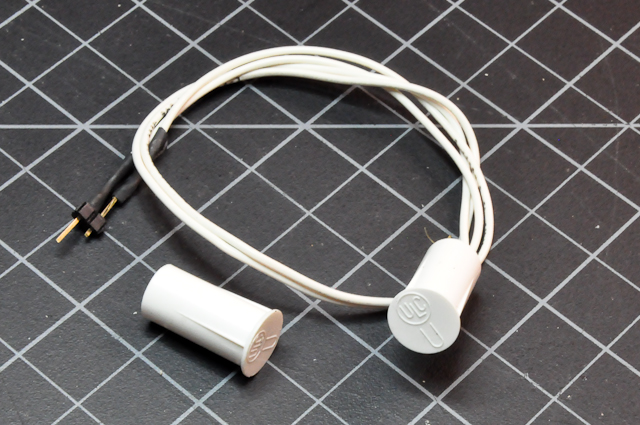
\includegraphics[scale=0.3]{img/switches/magnetic_switch.jpg}
 \caption{magnetic switch}
 \label{magnetic switch}
\end{figure}











\begin{figure}[!htb]
 \centering
 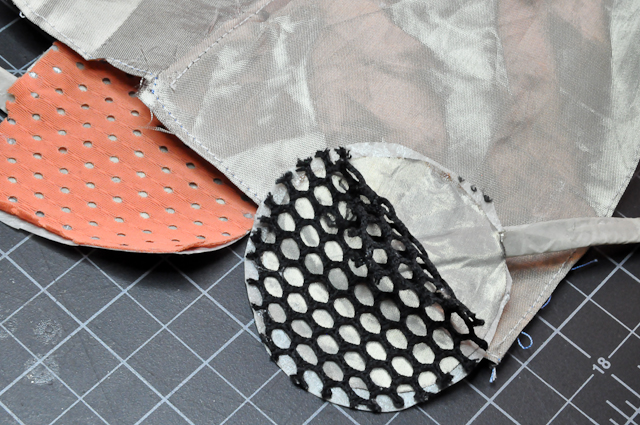
\includegraphics[scale=0.3]{img/switches/soft_switches.jpg}
 \caption{soft switches}
 \label{soft switches}
\end{figure}





\begin{figure}[!htb]
 \centering
 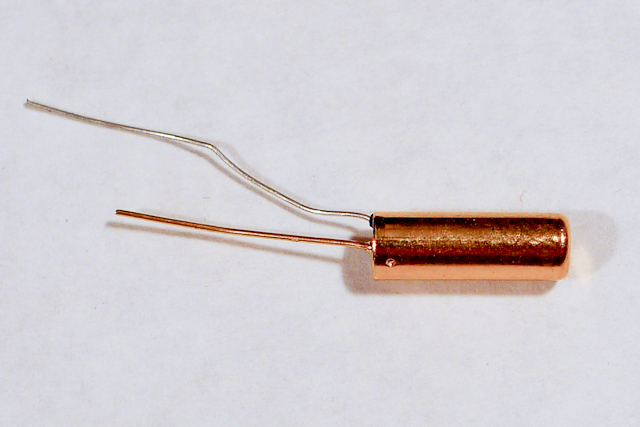
\includegraphics[scale=0.3]{img/switches/tilt_switch.jpg}
 \caption{tilt switch}
 \label{tilt switch}
\end{figure}





\begin{figure}[!htb]
 \centering
 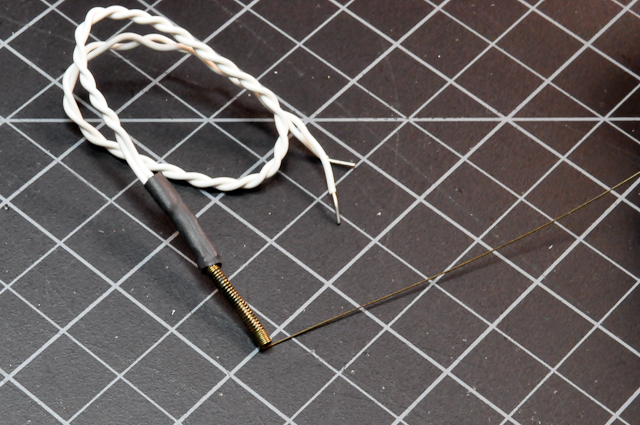
\includegraphics[scale=0.3]{img/switches/whisker_switch.jpg}
 \caption{whisker switch}
 \label{whisker switch}
\end{figure}


\begin{figure}[!htb]
 \centering
 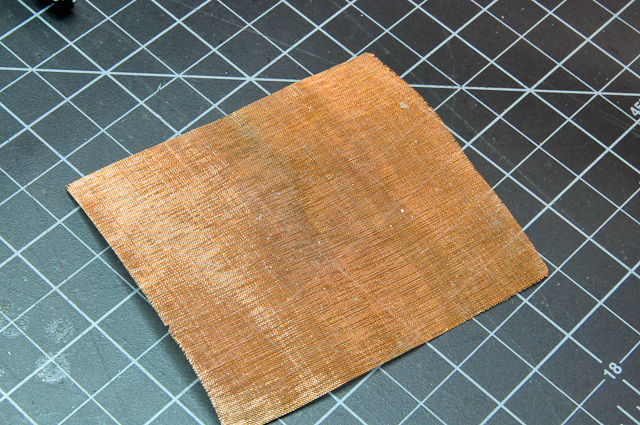
\includegraphics[scale=0.3]{img/switches/wire_mesh.jpg}
 \caption{wire mesh}
 \label{wire mesh}
\end{figure}


